


\section{Model Derivations}


\subsection{Firm First-order Conditions}
\subsubsection{Pricing}
Let $\eta$ be the Lagrange multiplier associated with the constraint $y_{j,t}=\left(\frac{p_{j,t}}{P_{t}}\right)^{-\frac{\mu_{p}}{\mu_{p}-1}}Y_{t}$. The first-order condition for prices $p_{j,t}$ is:
\begin{align*} 
\frac{\partial\mathcal{L}_{t}}{\partial p_{j,t}}=&\left(1-\tau^{c}\right)\left\{ \frac{y_{j,t}}{P_{t}}-\frac{\mu_{p}}{\mu_{p}-1}\frac{1}{\epsilon_{p}}\left[\ln\left(1+\pi_{j,t}\right)\right]Y_{t}\frac{1}{1+\pi_{j,t}}\frac{1}{p_{j,t-1}}\right. \\
&+\left.\frac{1}{1+r_{t+1}}\left[-\frac{\mu_{p}}{\mu_{p}-1}\frac{1}{\epsilon_{p}}\left[\ln\left(1+\pi_{j,t+1}\right)\right]Y_{t+1}\frac{1}{1+\pi_{j,t+1}}\left(-\frac{p_{j,t+1}}{p_{j,t}^{2}}\right)\right]\right\} \\
&-\eta_{t}\left[-\left(-\frac{\mu_{p}}{\mu_{p}-1}\right)\left(\frac{p_{j,t}}{P_{t}}\right)^{-\frac{\mu_{p}}{\mu_{p}-1}-1}\frac{Y_{t}}{P_{t}}\right]=0
\end{align*}
Define $mc_{t}\equiv 1-\frac{\eta_{t}}{1-\tau^{c}}$ and simplify, to get the forward looking, New Keynesian Philips curve:
\begin{align*} 
\ln\left(1+\pi_{j,t}\right)=\epsilon_{p}\left(mc_{t}-\frac{1}{\mu_{p}}\right)+\frac{1}{1+r_{t+1}}\left[\ln\left(1+\pi_{j,t+1}\right)\right]\frac{Y_{t+1}}{Y_{t}}
\end{align*}


\subsubsection{Capital Demand}
The first-order condition for capital is:
\begin{gather*}
\frac{\partial\mathcal{L}_{t}}{\partial k_{j,t}}=\left(1-\tau^{c}\right)\left\{ \frac{p_{j,t}}{P_{t}}\frac{\partial y_{j,t}}{\partial k_{j,t}}-r_{t}^{k}\right\} -\eta_{t}\left[\frac{\partial y_{j,t}}{\partial k_{j,t}}\right]=0 \\
\alpha\frac{Y_{t}}{K_{t}}mc_{t}=r_{t}^{k}
\end{gather*}


\subsubsection{Vacancy posting and labor demand}
The vacancy posting FOC is: 
\begin{align*}
\frac{\partial\mathcal{L}_{t}}{\partial v_{j,t}}=-\left(1-\tau^{c}\right)\epsilon_{L}+\Xi_{t}m_{t}=0 \\
\Leftrightarrow\left(1-\tau^{c}\right)\epsilon_{L}=\Xi_{t}m_{t}  
\end{align*}
The FOC for labor demand is:
\begin{gather*}
\frac{\partial\mathcal{L}_{t}}{\partial n_{j,t}}=\left(1-\tau^{c}\right)\left\{ \frac{p_{j,t}}{P_{t}}\frac{\partial y_{j,t}}{\partial l_{j,t}}-w_{t}\right\} -\eta_{t}\left[\frac{\partial y_{j,t}}{\partial l_{j,t}}\right]-\Xi_{t}+\frac{1}{1+r_{t+1}}\Xi_{t+1}\left(1-\delta^{\text{L}}\right)=0
\end{gather*}
Combining this, and the vacancy posting FOC gives:
\begin{gather*}
\left(1-\alpha\right)\frac{Y_{t}}{N_{t}}mc_{t}=w_{t}+\frac{\epsilon_{L}}{m_{t}}-\frac{\left(1-\delta^{\text{L}}\right)}{1+r_{t+1}}\frac{\epsilon_{L}}{m_{t+1}}    
\end{gather*}


\subsubsection{Capital firms - Capital supply}
Capital firms max the objective function:
\begin{align*}
V_{t}^{K}\left(K_{t-1},K_{t},I_{t-1},I_{t},I_{t+1}\right)=&\max_{K_{t},I_{t}}D_{t}^{K}\left(K_{t-1},I_{t-1},I_{t}\right)+p_{t}^{K}\left(K_{t},I_{t},I_{t+1}\right) \\
&+\frac{1}{1+r_{t+1}}V_{t+1}^{K}\left(K_{t},K_{t+1},I_{t},I_{t+1},I_{t+2}\right)
\end{align*}
subject to capital accumulation $K_{t}=\left(1-\delta\right)K_{t-1}+Z_{t}^{I}I_{t}$, and where dividends are given by:
\begin{gather*}
D_{t}^{K}\left(K_{t-1},I_{t-1},I_{t}\right)=r_{t}^{k}K_{t-1}-I_{t}\left(1+\phi_{I}\left(\frac{I_{t}}{I_{t-1}}\right)\right)
\end{gather*}
and the dividend price $p^K$ is given by:
\begin{gather*}
p_{t}^{K}\left(K_{t},I_{t},I_{t+1}\right)=\frac{1}{1+r_{t+1}}\left[D_{t+1}^{K}\left(K_{t},I_{t},I_{t+1}\right)+p_{t+1}^{K}\left(K_{t+1},I_{t+1},I_{t+2}\right)\right]
\end{gather*}


The first-order condition for investment $I_t$ is:
\begin{gather*}
\frac{\partial D_{t}^{K}\left(K_{t-1},I_{t-1},I_{t}\right)}{\partial I_{t}}+\frac{\partial p_{t}^{K}\left(K_{t},I_{t},I_{t+1}\right)}{\partial I_{t}}=0 \\
\Leftrightarrow\frac{\partial D_{t}^{K}\left(K_{t-1},I_{t-1},I_{t}\right)}{\partial I_{t}}+\frac{\partial p_{t}^{K}\left(K_{t},I_{t},I_{t+1}\right)}{\partial I_{t}}+\frac{\partial p_{t}^{K}\left(K_{t},I_{t},I_{t+1}\right)}{\partial K_{t}}\frac{\partial K_{t}}{\partial I_{t}}=0,
\end{gather*}
The derivative $\frac{\partial p_{t}^{K}\left(K_{t},I_{t},I_{t+1}\right)}{\partial I_{t}}$ can be derived as:
\begin{align*}
\frac{\partial p_{t}^{K}\left(K_{t},I_{t},I_{t+1}\right)}{\partial I_{t}}&=\frac{1}{1+r_{t+1}}\left[-\frac{\partial I_{t+1}\phi_{I}\left(\frac{I_{t+1}}{I_{t}}\right)}{\partial I_{t}}\right] \\
&=\frac{1}{1+r_{t+1}}\phi_{I}'\left(\frac{I_{t+1}}{I_{t}}\right)\left(\frac{I_{t+1}}{I_{t}}\right)^{2}
\end{align*}
Defining $Q_{t} \equiv \frac{\partial p_{t}^{K}\left(K_{t},I_{t},I_{t+1}\right)}{\partial K_{t}}$ and using the above yields the first equation:
\begin{gather*}
1+\frac{I_{t}}{I_{t-1}}\phi_{I}'\left(\frac{I_{t}}{I_{t-1}}\right)+\phi_{I}\left(\frac{I_{t}}{I_{t-1}}\right)=Q_{t}Z_{t}^{I}+\frac{1}{1+r_{t+1}}\phi_{I}'\left(\frac{I_{t+1}}{I_{t}}\right)\left(\frac{I_{t+1}}{I_{t}}\right)^{2}
\end{gather*}

The first-order condition for capital is:
\begin{gather*}
\frac{\partial p_{t}^{K}\left(K_{t},I_{t},I_{t+1}\right)}{\partial K_{t}}=\frac{1}{1+r_{t+1}}\left[r_{t+1}^{k}+\frac{\partial p_{t+1}^{K}\left(K_{t+1},I_{t+1},I_{t+2}\right)}{\partial K_{t}}\right] \\
\Leftrightarrow Q_{t}=\frac{1}{1+r_{t+1}}\left[r_{t+1}^{k}+Q_{t+1}\left(1-\delta\right)\right]
\end{gather*}










\subsection{Model:}
\begin{gather}
  \ln\left(1+\pi_{j,t}\right)=\epsilon_{p}\left(mc_{t}-\frac{1}{\mu_{p}}\right)+\frac{1}{1+r_{t+1}}\left[\ln\left(1+\pi_{j,t+1}\right)\right]\frac{Y_{t+1}}{Y_{t}} \\ \eqname{NKPC} \\
 \alpha\frac{Y_{t}}{K_{t}}mc_{t}=r_{t}^{k} \\ \eqname{Capital demand FOC} \\
  \left(1-\alpha\right)\frac{Y_{t}}{N_{t}}mc_{t}=w_{t}+\frac{\epsilon_{L}}{m_{t}}-\frac{\left(1-\delta^{\text{L}}\right)}{1+r_{t+1}}\frac{\epsilon_{L}}{m_{t+1}}   \label{abc} \\ \eqname{Vacancy/labor FOC} \\
div_{t}=Y_{t}-w_{t}L_{t}-\kappa_{V}V_{t}-r_{t}^{k}K_{t}-\Phi^{P}\left(P_{t},P_{t-1}\right)  \\ \eqname{Firm dividends}   \\
  w_{t}=w^{ss}\left(\frac{Y_{t}/N_{t}}{Y_{t}^{ss}/N_{t}^{ss}}\right)^{\eta},  \\ \eqname{Wage function}  \\
  K_{t}=\left(1-\delta^{K}\right)K_{t-1}+I_{t} \\ \eqname{Capital LOM}  \\
  N_{t}=\left(1-\delta^{\text{L}}\right)N_{t-1}+m_{t}V_{t} \\ \eqname{Employment LOM}  \\
  M_{t}=S_{t}^{\xi}V_{t}^{1-\xi}   \\ \eqname{Matching Function}  \\
  V_{t}m_{t}=q_{t}S_{t}  \\ \eqname{New Matches}  \\
  \tau^{VAT}C_{t}+(\tau^{c}+\tau^{div})div_{t}+\tau^{div}div_{t}^{MF}A_{t}+T^{I}\left(w,N\right)+B_{t} \\
=G_{t}+bU_{t}+T_{t}+B_{t-1}\left(1+r_{t}\right). \\ \eqname{Government Budget}  \\
i_{t}=\max\left\{ 0,i^{*}+\left(\phi^{MP}-1\right)\pi_{t}+\mathbb{E}_{t}\pi_{t+1}\right\} \\ \eqname{Taylor Rule}  \\
1+r_{t}=\frac{1+i_{t-1}}{1+\pi_{t}} \\ \eqname{Fisher eq.}  \\
A_{t}^{*}\left(r_{t},w_{t},N_{t},q_{t}\right) \\ \eqname{Asset policy function}   \\
C_{t}^{*}\left(r_{t},w_{t},N_{t},q_{t}\right) \\ \eqname{Consumption function}    
\end{gather}
\begin{gather}
Q_{t}\left(1-\kappa_{I}\left(\frac{I_{t}}{I_{t-1}}-1\right)\frac{I_{t}}{I_{t-1}}-\frac{\kappa_{I}}{2}\left(\frac{I_{t}}{I_{t-1}}-1\right)^{2}\right) \notag \\
= -Q_{t+1}\kappa_{I}\left(\frac{I_{t+1}}{I_{t}}-1\right)\left(\frac{I_{t+1}}{I_{t}}\right)^{2} \\ \eqname{Mut. fund Investment FOC}   \\
 \left(1+r_{t}^{k}-\delta^{k}\right)=\left(1+\tilde{r}_{t}^{a}\right)+Q_{t}-Q_{t+1}\left(1-\delta^{k}\right) \\ \eqname{Mut. fund Capital FOC}   \\
div_{t}^{MF}=\left(1+r_{t}^{k}-\delta\right)\frac{K_{t}}{A_{t}}+\left(1+r_{t}\right)\frac{B_{t}}{A_{t}}-\left(1+r_{t}\right)    \\ \eqname{Mut. fund dividends}   \\
\end{gather}
 
 
 
%\bgroup
%\def\arraystretch{1.3}
%\setlength{\tabcolsep}{1.1em} 
%\begin{table}[H]\centering \footnotesize
%\caption{Solution Error - Euler errors } 
%\label{table:Euler_errors}
%\makebox[\textwidth]{ 
%\begin{tabular}{l*{3}{c}}
%\hline\hline
%            & \multicolumn{1}{c}{Employed} & \multicolumn{1}{c}{Unemployed}    \\
%\hline 
%{Average}   & -3.505 & -3.205  \\  
%{Max}       & -2.505  & -2.460   \\ 
%\hline\hline 
%\multicolumn{3}{l}{\footnotesize The table shows the average and maximum Euler errors computed as %$\overline{\mathcal{E}}&\equiv\frac{\mathcal{D}^{ss}\cdot\mathcal{E}\mathbf{1}_{a>\epsilon}}{\mathcal{D}^{ss}\cdot\mathbf{1}_{a>\epsilon}}$ where $\mathcal{E}$ is a vector whose $i$th entry is given by %$\mathcal{E}_{i}&\left.\equiv\log_{10}\left(\left|\Delta_{i}/c_{i}\right|\right)\right)$
%denotes relative (percentage) change.   }\\
%\end{tabular}
%}
%\end{table}



\section{Consumption Analysis} 

\begin{figure}[H]
\makebox[\linewidth][c]{%
  \centering
  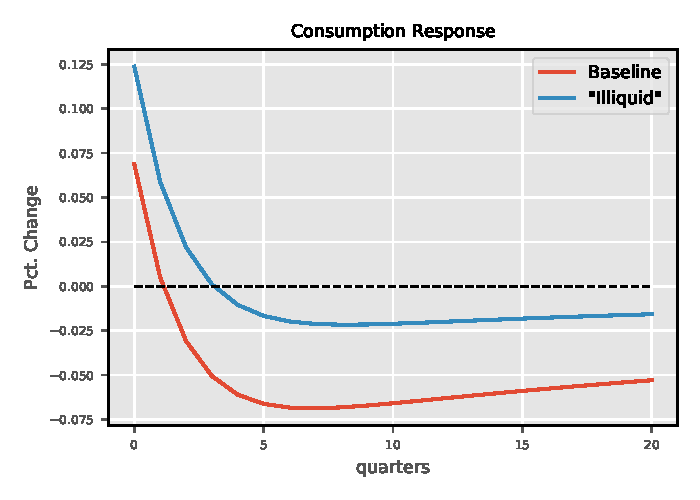
\includegraphics[width=.5\linewidth]{mainmatter/plots/SS_evaluation/Alternative_calibs/Consumption_interest_rate_response_agg_illiquid.pdf}
  }
     \caption{Responses with "illiquid" assets (reduced unhedged interest rate exposure).}
\label{fig:dC_dR_illiquid_example}
\end{figure}



\subsection{Robustness check: Household Parameters} \label{sec:C_robustness}
The responses of consumption to changes in income and the interest rate are central to the impulse responses of the model. In the standard RANK setup the household setup is sufficiently transparent such that the implication of different parameterizations are relatively easy to analyze and test. In models with heterogeneous consumers a similar robustness check is more complicated since a change in a given parameter, say, the intertemporal elasticity of substitution $\sigma$ (EIS), has two effects: 1) A different EIS affects the curvature of the Euler equation hence affecting the dynamic consumption response shape, and 2) A different EIS affect the amount of assets individuals choose to hold in steady-state, and hence the wealth distribution changes. To overcome the interplay between these two channels I do the following: To investigate the effect of the first channel I consider the change in aggregate consumption $dC$ calculated as $\sum_{i}\mathcal{D}_{i,t}^{Base}c_{i,t}$ where $\sum_{i}d\mathcal{D}_{i,t}^{Base}dc_{i,t}$ is the distribution matrix from the \textit{baseline} calibration and $dc_{i,t}$ is the change in individual consumption under the alternative parameterization. Hence I avoid distributional effects from parameter changes by fixing the distribution to the one from the baseline calibration.\footnote{keeping the distribution $\mathcal{D}$ fixed is not sufficient to match the exact same steady-state distribution since asset levels can change endogenously, but it does ensure that the distributions are very similar. Still, the marginal differences can have large effects if they change the number of constrained consumers significantly. To avoid this, I compute a reshuffling of $\mathcal{D}$ by removing a small share of consumers $\epsilon$ of the constrained consumers and adding them uniformly to all other groups with the aim being the same share of constrained consumers as in the baseline.  } \\


Figure \ref{fig:calibration_C_r_eis} shows the consumption (MPC) responses to the earlier described income and interest rate shocks (i.e. the partial equilibrium responses) for different values of the intertemporal elasticity of substitution, with $\sigma=0.5$ being the baseline value. The figure reveals that, conditional on wealth and income distributions, the dynamic consumption response is very sensitive to the choice of the EIS. Recall that a higher EIS imply less curvature in the utility of consumption, with the limiting cases $\sigma\rightarrow0,\sigma\rightarrow\infty$ corresponding to current and future consumption being perfect complements and perfect substitutes respectively. 
For the income shock a higher EIS imply that households spend more of the transitory income gain today, with the result being a higher contemporaneous MPC, and higher persistence. For the interest rate shock, the response becomes signficantly more volatile as the elasticity increases since households are more willing to substitute between current and future consumption. Neither of the EIS parametriations match the response from \citet{kaplan2018monetary}, which resembles more closely the RANK response. \\

Figure \ref{fig:calibration_C_r_std} shows the effect of varying the standard deviation of the earnings process. Note that since the standard deviation determines income dispersion it primarily affects the model through the wealth distribution, which is kept fixed here. The remaining effect from the earnings dispersion is marginal: MPCs are roughly invariant towards the dispersion, while for the interest rate shock it primarily matters for the long run persistence of the shock. The marginal differences here could, however, be due to slight changes in the wealth distribution.  \\
% Hmm this shock is proably a bit wierd???? 


\begin{figure}[H]

\centering
\begin{subfigure}{.9\textwidth}
  \centering
  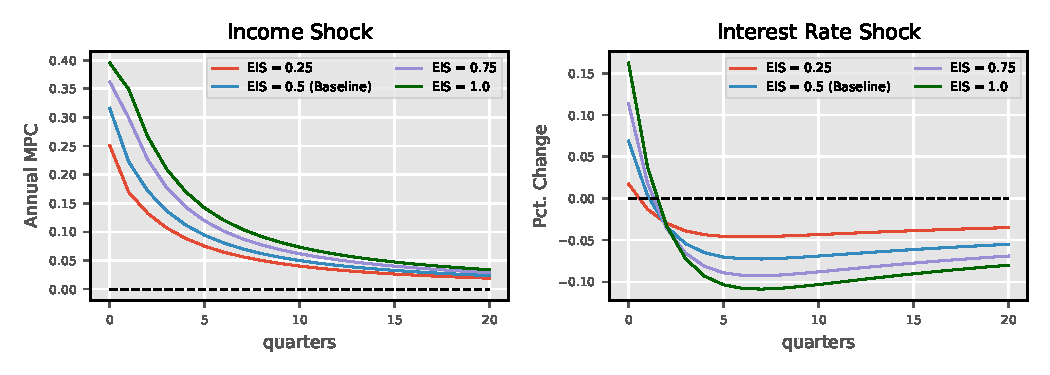
\includegraphics[width=.98\linewidth]{mainmatter/plots/SS_evaluation/Alternative_calibs/C_R_earnings_EIS.pdf} 

  \caption{Varying the intertemporal elasticity of substitution. \label{fig:calibration_C_r_eis} } 
\end{subfigure}

\begin{subfigure}{.9\textwidth}
  \centering
  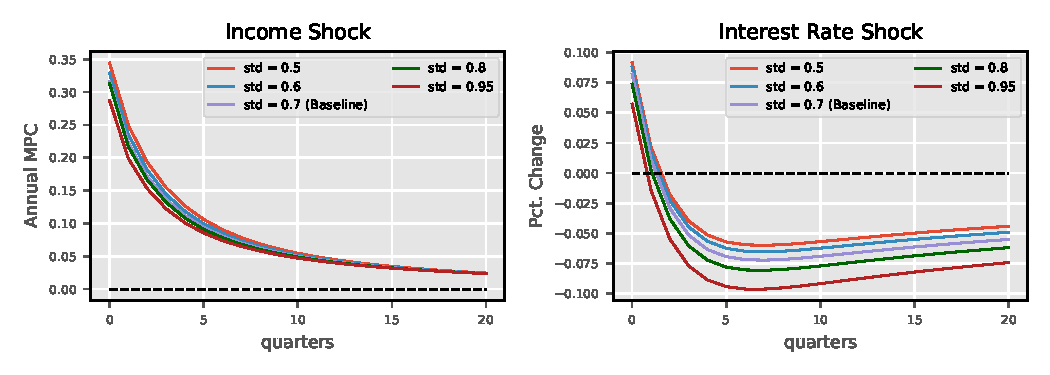
\includegraphics[width=.98\linewidth]{mainmatter/plots/SS_evaluation/Alternative_calibs/C_R_earnings_std.pdf} 
  \caption{Varying the standard deviation of earnings. }  \label{fig:calibration_C_r_std}
\end{subfigure}

\caption{Consumption responses to income and interest rate shocks under various calibrations.}
\label{fig:dC_robust}
\end{figure}


%\subsection{Reflection} % Job finding rate response. 
%I have so far considered how consumption reacts to changes in disposable income and interest rates, which are the two primarily channels that may affect consumption. Consider for a moment how each of these channels are affected by the business cycle. 

% C makes up roughly half of Y in DK 
% more volatile than GDP, but 1/3 as volatile as I. However I share of Y is 16%. 


%In typical NK models changes in disposable income are generated by changes in wages, employment, lump sum transfers and, potentially, dividends. Wages are usually considered very rigid, almost acyclical, and dividends are modeled as firm equity, not transfers. Hence it is mostly employment and lump sum transfers that can move disposable income and hence consumption. As per the exposition above, interest rates affect consumption, but probably not enough to account for the aggregate volatility observed. What remains to affect consumption decisions is essentially precautionary savings, i.e. the fact that households increase savings by cutting consumption when faced with an increase in risk. In the present model the only source of cyclical risk is through the labor market job-finding rates. 


%The remaining channel affecting consumption is not related to income or financial flows but rather behavior and expectations. In
% Add section analyzing finding rates? 


\begin{figure}[H]
\centering
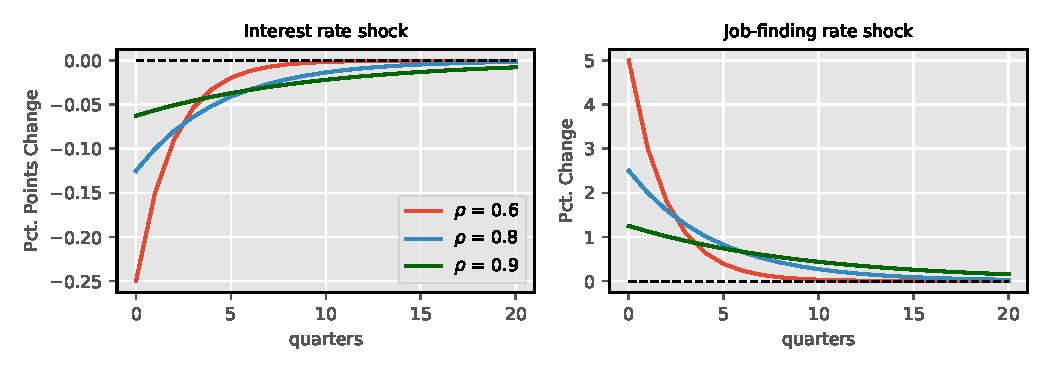
\includegraphics[width=.98\linewidth]{mainmatter/plots/C_analysis/ra_q_shocks.pdf} 
\caption{Shocks to interest- and job-finding rates with differing AR coefficient $\rho$.}
\label{fig:ra_q_shocks}
\end{figure}


\subsection{Aggregation Result: Proof} \label{Agg_result_proof}
% Assume
% no wage changes -> fixed labor suuply since no waelth effect
% borrowing constraint at zero 
% igonore  VAT - does not matter 
As in the main text I consider the aggregate change in consumption $dC_{t}=\int dc_{t}^{*}d\mathcal{D}_{ss}+\int c_{ss}^{*}d\mathcal{D}_{t}$, and specifically the term $\int dc_{t}^{*}d\mathcal{D}_{ss}$. Since we condition on the steady-state distribution of households the share of constrained households $\lambda$ is fixed. Let $c_{t}^{R}$ denote consumption of non-constrained ("Ricardian") agents and $c_{t}^{HtM}$ consumption of constrained ("Hand-to-Mouth") agents. Then:
\begin{gather*}
\int dc_{t}^{*}d\mathcal{D}_{ss}=\left(1-\lambda\right)\int dc_{t}^{R}d\mathcal{D}_{ss}^{R}+\lambda\int dc_{t}^{HtM}d\mathcal{D}_{ss}^{HtM}
\end{gather*}
The budget constraint for a constrained household is:
\begin{gather*}
c_{i,t}^{HtM}+\underline{a}=(1+r_{t}^{a})a_{i,t-1}+I_{i,t}-\tau^{I}\left(I_{i,t}\right)+T_{t}
\end{gather*}
Assume that wages are fixed and consider a first-order perturbation:
\begin{gather*}
dc_{i,t}^{HtM}=(1+r_{ss}^{a})da_{i,t-1}+\underline{a}dr_{t}^{a}+dT_{i,t}
\end{gather*}
since $a_{i,t-1}$ is fixed when conditioning on the initial distribution we have $da_{i,t-1}=0$ such that $dc_{i,t}^{HtM}=\underline{a}dr_{t}^{a}+dT_{i,t}$, which obliviously aggregates:
\begin{gather*}
\int dc_{i,t}^{HtM}d\mathcal{D}_{ss}^{HtM}=\int\underline{a}dr_{t}^{a}d\mathcal{D}_{ss}^{HtM}+\int dT_{i,t}d\mathcal{D}_{ss}^{HtM} \\
\Leftrightarrow dC_{t}^{HtM}=\underline{a}dr_{t}^{a}+dT_{t}
\end{gather*}
Rational household obey the linearized Euler equation:
\begin{gather*}
dc_{i,t}^{R}=\beta_{i}R_{ss}\left(E_{i,t}dc_{i,t+1}^{R}-\sigma R_{t+1}c_{i,ss}^{R}\right)
\end{gather*}
This disregards unemployment risk since I do not consider shock to the separation rate or the job-finding rate in this setting. Aggregating yields:
\begin{gather*}
\int dc_{i,t}^{R}d\mathcal{D}_{ss}=\int\beta_{i}R_{ss}\left(E_{i,t}dc_{i,t+1}^{R}-\sigma R_{t+1}c_{i,ss}^{R}\right)d\mathcal{D}_{ss} \\
\Leftrightarrow dC_{t}^{R}=R_{ss}\int\beta_{i}E_{i,t}dc_{i,t+1}^{R}d\mathcal{D}_{ss}-\sigma R_{t+1}C_{ss}^{R}
\end{gather*}


\subsection{Details on RA/TA household models} \label{sec:RA_TA}
\subsubsection{Canonical RA model.}
Assuming the representative family construct of \citet{merz1995search} implies that there is no idiosyncratic risk or unemployment risk. Hence only aggregate uncertainty matters, which there is none-off in the baseline model. The representative agent solves:
\begin{gather*}
V_{t}=\max_{C_{t}^{R},A_{t},\ell_{t}}\frac{C_{t}^{R}^{1-\frac{1}{\sigma}}}{1-\frac{1}{\sigma}}-\varphi\frac{\ell_{t}^{1+\frac{1}{\varphi}}}{1+\frac{1}{\varphi}}+\beta\mathbb{E}_{t}V_{t+1} \\
s.t.\\
\left(1+\tau^{c}\right)C_{t}^{R}+A_{t}=\left(1+r\right)A_{t-1}+I_{t}+T_{t}-\tau\left(I_{t}\right),
\end{gather*}
where $I_{t}=w_{t}\ell_{t}N_{t}+b_{t}\left(1-N_{t}\right)$. This results in the standard consumption Euler equation $\left(C_{t}^{R}\right)^{-\frac{1}{\sigma}}=R_{t+1}\beta\left(C_{t+1}^{R}\right)^{-\frac{1}{\sigma}}$.

\subsubsection{Canonical TA model.}
The canonical two-agent household model of \citet{campbell1989consumption} assumes that a fraction $\lambda$ of households obey a rule-of-thumb of consuming their entire income each period, and hence holds no assets. Consumption obeys:
\begin{gather*}
C_{t}^{HtM}=\frac{1}{1+\tau^{c}}\left(\lambda I_{t}-\tau\left(\lambda I_{t}\right)+\lambda T_{t}\right), \\
C_{t}=C_{t}^{R}+C_{t}^{HtM},
\end{gather*}
where $C_{t}^{R}$ is defined as above in the RA's problem, but with income flows scaled by the share of Ricardian agents $1-\lambda$.


%\subsubsection{TA model with Unemployment Risk.} 
%I assume that there is perfect insurance against idiosyncratic earnings risk but not unemployment risk. Consumption of hand-to-mouth consumers is unchanged but for Ricardian agents there now exists a representative household for employed and unemployed. Hence the model actually contains three representative agents. Consumption for the two Ricardian households obey:
%\begin{gather*}
%\left(C_{t}^{N,R}\right)^{-\frac{1}{\sigma}}=R_{t+1}\beta\left[\left(1-\delta\left(1-q_{t+1}\right)\right)\left(C_{t+1}^{N,R}\right)^{-\frac{1}{\sigma}}+\delta\left(1-q_{t+1}\right)\left(C_{t+1}^{U,R}\right)^{-\frac{1}{\sigma}}\right], \\
%\left(C_{t}^{U,R}\right)^{-\frac{1}{\sigma}}=R_{t+1}\beta\left[q_{t+1}\left(C_{t+1}^{N,R}\right)^{-\frac{1}{\sigma}}+\left(1-q_{t+1}\right)\left(C_{t+1}^{U,R}\right)^{-\frac{1}{\sigma}}\right]
%\end{gather*}
%where budget constraints associated with each state is:
%\begin{gather*}
%\left(1+\tau^{c}\right)C_{t}^{N,R}+A_{t}^{N}=\left(1+r\right)A_{t-1}^{N}+w_{t}\ell_{t}+T_{t}-\tau\left(w_{t}\ell_{t}\right), \\
%\left(1+\tau^{c}\right)C_{t}^{U,R}+A_{t}^{U}=\left(1+r\right)A_{t-1}^{U}+b_{t}+T_{t}-\tau\left(b_{t}\right)
%\end{gather*}
%Aggregate consumption for Ricardian agents is $C_{t}^{R}=N_{t}C_{t}^{N,R}+\left(1-N_{t}\right)C_{t}^{U,R}$.




\begin{figure}[H]
\makebox[\linewidth][c]{%
\centering
  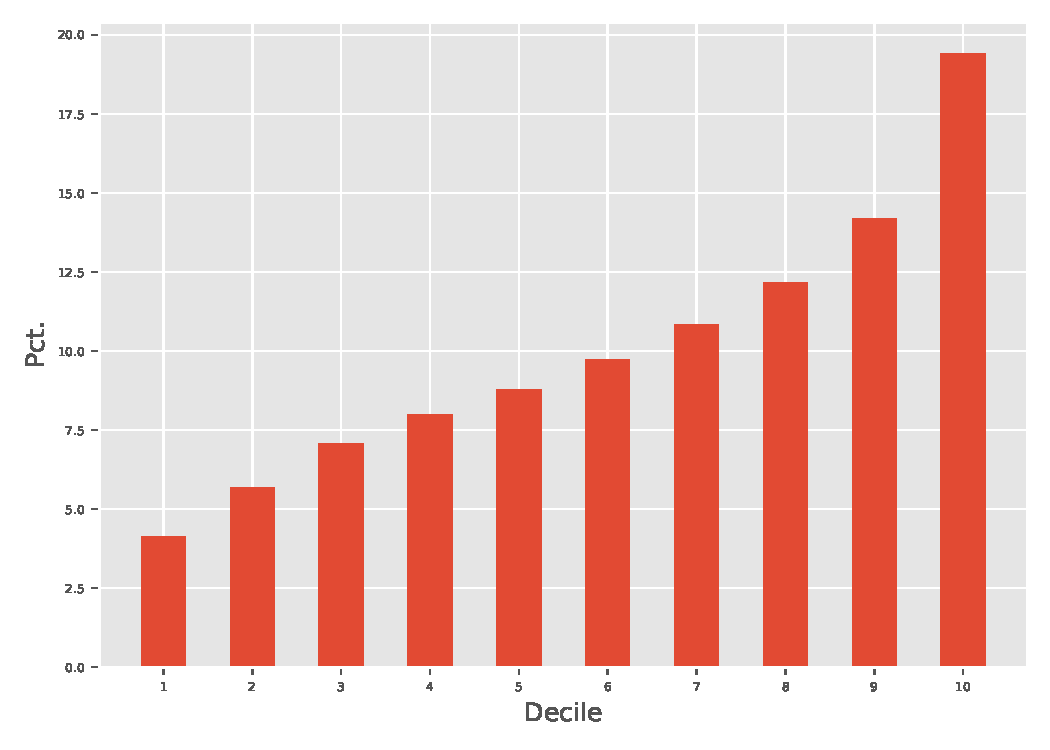
\includegraphics[width=.5\linewidth]{mainmatter/plots/SS_evaluation/C_by_deciles.pdf} 
}
\caption[Caption for LOF]{Distribution of consumption over wealth deciles in steady-state.}
\label{fig:C_dist_by_deciles}
 % {\scriptsize  Impulse responses to a negative productivity shock of 1\% with persistence 0.94 (half-life: 5 quarters). }
\end{figure}



\begin{figure}[H]
\makebox[\linewidth][c]{%
\centering
  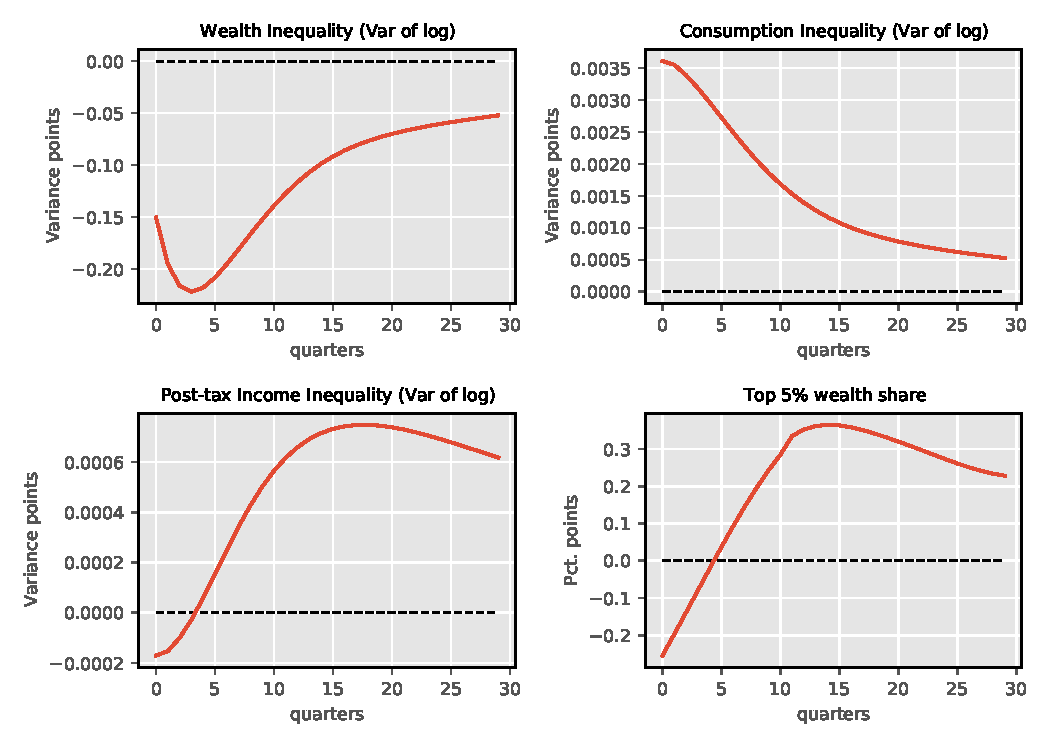
\includegraphics[width=.8\linewidth]{mainmatter/plots/SS_evaluation/TFP_shock_inequality.pdf} 
}
\caption[Caption for LOF]{Inequality responses following TFP shock.}
\label{fig:Inequality_response}
\centering
 {\scriptsize  Note: The first three panels measure wealth, consumption and income inequality over the cycle by the change in the variance of the log distribution relative to steady-state. The final panel computes the change in the wealth share of the top 5\% wealthiest households relative to steady-state.  }
\end{figure}


\section{Automatic Stabilizers- Unemployment Benefits}

\begin{figure}[H]
\makebox[\linewidth][c]{%
\centering
  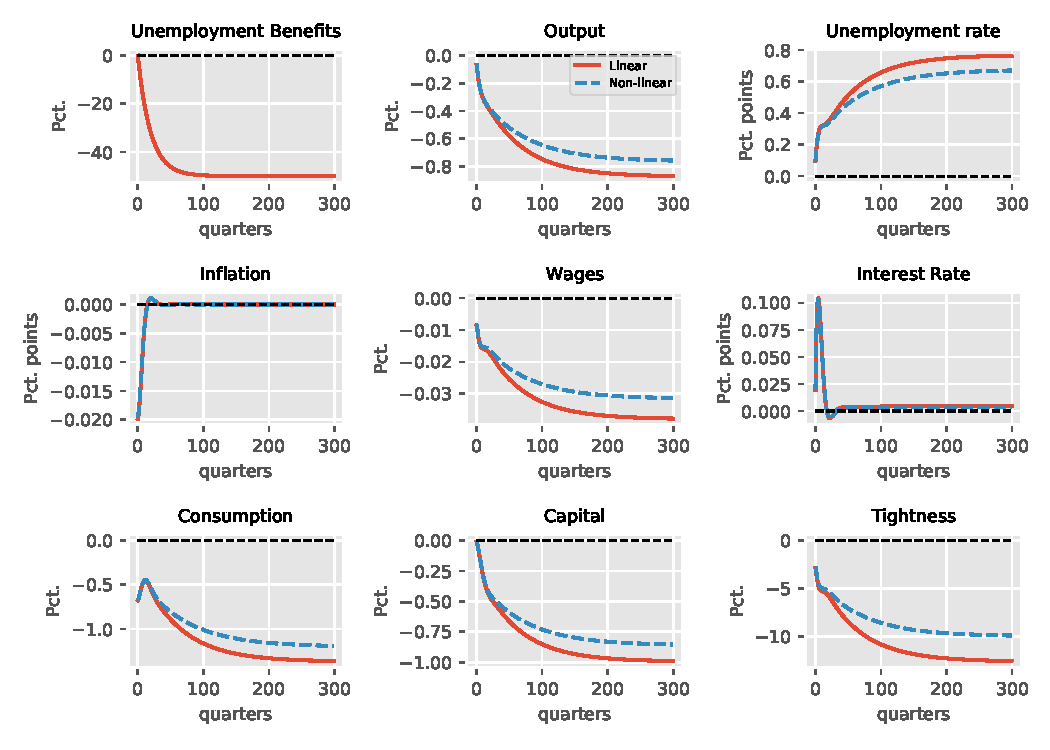
\includegraphics[width=.98\linewidth]{mainmatter/plots/Lower_b_main/transition_to_new_ss_non_linear_comp.pdf} 
}
\caption[Caption for LOF]{Transitional Dynamics following a lower unemployment benefit rate - linear and non-linear impulses.}
\label{fig:Lower_b_Transitional}
 % {\scriptsize  Impulse responses to a negative productivity shock of 1\% with persistence 0.94 (half-life: 5 quarters). }
\end{figure}



\begin{figure}[H]
\makebox[\linewidth][c]{%
\centering
  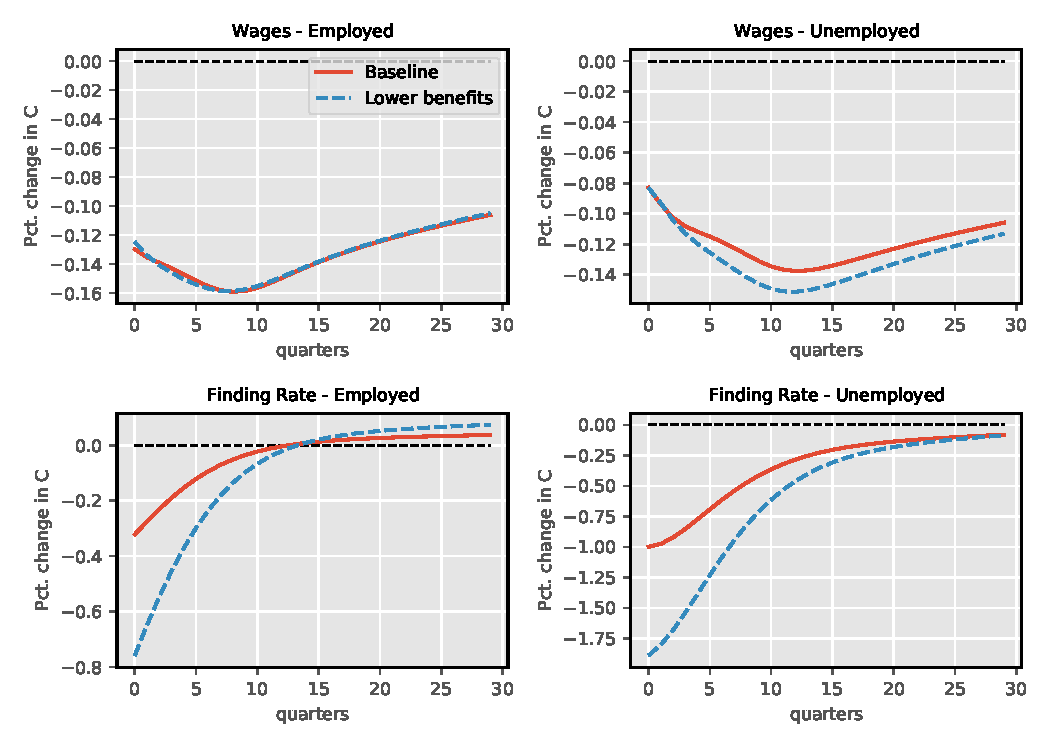
\includegraphics[width=.8\linewidth]{mainmatter/plots/Lower_b_main/main_result_C_decomp_N_U_G.pdf} 
}
\caption[Caption for LOF]{Effect on consumption from wages and job finding rate by employment status - financed by cutting government spending.}
\label{fig:lower_b_C_decomp_by_N_G}
 % {\scriptsize  Impulse responses to a negative productivity shock of 1\% with persistence 0.94 (half-life: 5 quarters). }
\end{figure}


\begin{figure}[H]
\makebox[\linewidth][c]{%
\centering
  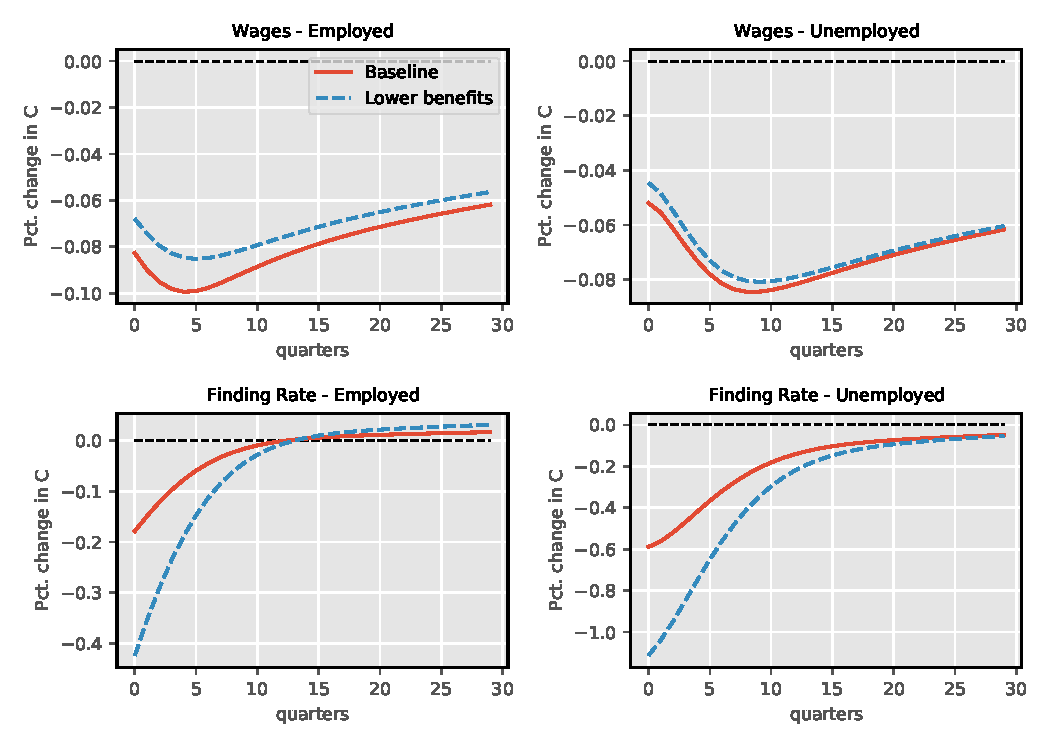
\includegraphics[width=.8\linewidth]{mainmatter/plots/Lower_b_main/main_result_C_decomp_N_U_T.pdf} 
}
\caption[Caption for LOF]{Effect on consumption from wages and job finding rate by employment status - financed by cutting transfers.}
\label{fig:lower_b_C_decomp_by_N_T}
 % {\scriptsize  Impulse responses to a negative productivity shock of 1\% with persistence 0.94 (half-life: 5 quarters). }
\end{figure}



\begin{figure}[H]
\makebox[\linewidth][c]{%
\centering
  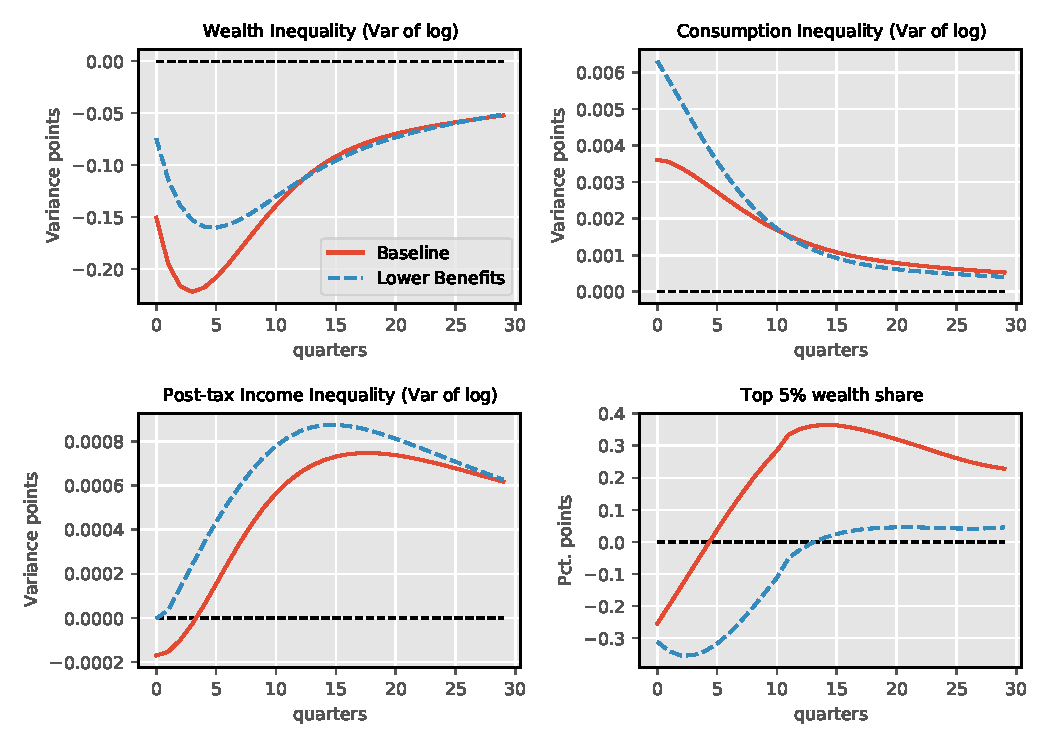
\includegraphics[width=.8\linewidth]{mainmatter/plots/Lower_b_main/agg_inequality_lower_b_G.pdf} 
}
\caption[Caption for LOF]{Inequality responses following TFP shock - comparison between baseline and model with lower unemployment benefits.}
\label{fig:Inequality_response_lower_b}
\centering
 {\scriptsize  Note: The first three panels measure wealth, consumption and income inequality over the cycle by the change in the variance of the log distribution relative to steady-state. The final panel computes the change in the wealth share of the top 5\% wealthiest households relative to steady-state.  }
\end{figure}
